In this lecture, we will apply our derivative machinery to a new type of input: neither scalars, nor column vectors, nor matrices, but rather the \textbf{inputs will be functions} $u(x)$, which form a perfectly good vector space (and can even have norms and inner products).\footnote{Being fully mathematically rigorous with vector spaces of functions requires a lot of tedious care in specifying a well-behaved set of functions, inserting annoying caveats about functions that differ only at isolated points, and so forth. In this lecture, we will mostly ignore such technicalities---we will implicitly assume that our functions are integrable, differentiable, etcetera, as needed.  The subject of \emph{functional analysis} exists to treat such matters with more care.}  It turns out that there are lots of amazing applications for differentiating with respect to \emph{functions}, and the resulting techniques are sometimes called the ``calculus of variations'' and/or ``Frech{\'{e}}t'' derivatives.


\subsection{Functionals: Mapping functions to scalars}

\begin{example}
For example, consider functions $u(x)$ that map $x\in [0,1] \to u(x) \in \R$.  We may then define the function $f$:
\[
f(u) = \int_0^1 \sin (u(x)) \,\mathrm{d} x.
\]
Such a function, mapping an input \emph{function} $u$ to an output \emph{number}, is sometimes called a ``functional.''  What is $f'$ or $\nabla f$ in this case?
\end{example}



Recall that, given any function $f$, we always define the derivative as a linear operator $f'(u)$ via the equation:
\[
\d f = f (u + \d u ) - f(u) = f'(u) [\d u] \, ,
\]
where now $\d u$ denotes an arbitrary ``small-valued'' \emph{function} $\d u(x)$ that represents a small change in $u(x)$, as depicted in Fig.~\ref{fig:du} for the analogous case of a non-infinitesimal $\delta u(x)$.
Here, we may compute this via linearization of the integrand: 
\begin{align*}
    \d f &= f(u+ \d u) - f(u) \\ 
     &=\int_0^1 \sin (u(x) + \d u(x)) - \sin (u(x)) \, \d x \\
     &= \int_0^1 \cos (u(x)) \, \d u(x) \, \d x = f'(u) [\d u] \, ,
\end{align*}
where in the last step we took $\d u(x)$ to be arbitrarily small\footnote{Technically, it only needs to be small ``almost everywhere'' since jumps that occur only at isolated points don't affect the integral.} so that we could linearize $\sin(u + \d u)$ to first-order in $\d u(x)$.  That's it, we have our derivative $f'(u)$ as a perfectly good linear operation acting on $\d u$!


\begin{figure}
    \centering
    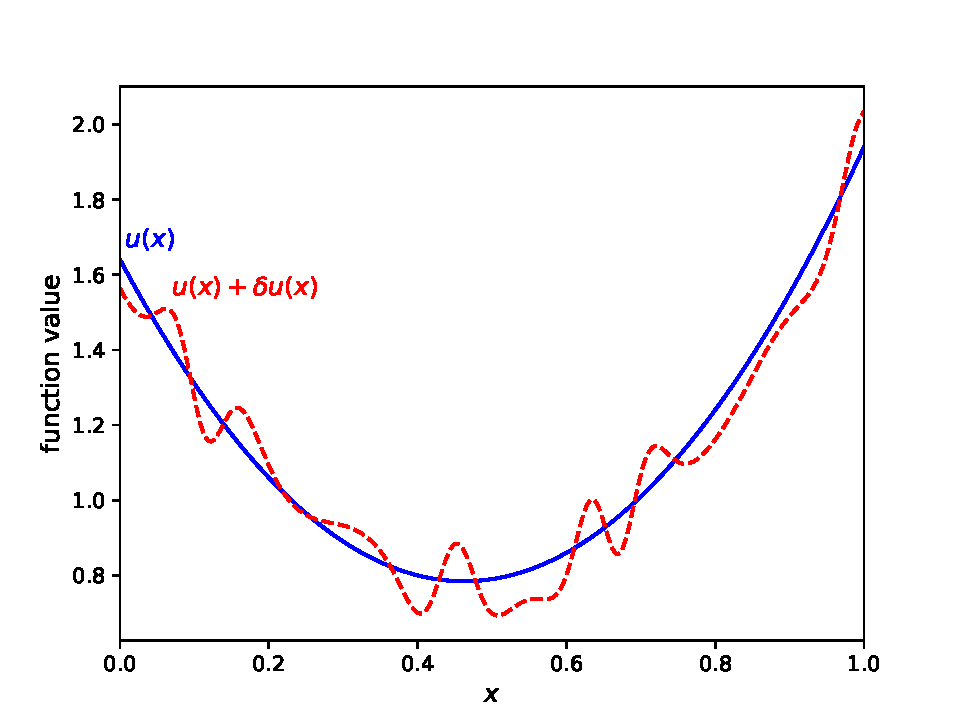
\includegraphics[width=0.6\textwidth]{figures/du}
    \caption{If our $f(u)$'s inputs $u$ are \emph{functions} $u(x)$ (e.g., mapping $[0,1] \mapsto \mathbb{R}$), then the essence of differentiation is linearizing $f$ for small perturbations $\delta u(x)$ that are themselves functions, in the limit where $\delta u(x)$ becomes arbitrarily small.  Here, we show an example of a $u(x)$ and a perturbation $u(x)+\delta u(x)$.}
    \label{fig:du}
\end{figure}

\subsection{Inner products of functions}

In order to define a gradient $\nabla f$ when studying such ``functionals'' (maps from functions to $\R$), it is natural to ask if there is an inner product on the input space. In fact, there are perfectly good ways to define inner products of functions! Given functions $u(x), v(x)$ defined on $x\in [0,1]$, we could define a ``Euclidean'' inner product:
\[
\langle u, v \rangle = \int_0^1 u(x) v(x) \,\mathrm dx.
\]
Notice that this implies 
\[
\lVert u \rVert := \sqrt{\langle u, u \rangle} = \sqrt{\int_0^1 u(x)^2 dx} \, .
\]

Recall that the gradient $\nabla f$ is \emph{defined} as whatever we take the inner product of $\d u$ with to obtain $\d f$. 
 Therefore, we obtain the gradient as follows: 
\[
\d f = f'(u)[\d u]  = \int_0^1 \cos(u(x)) \,\d u(x)\, \d x  = \langle \nabla f, \d u \rangle \implies \nabla f = \cos (u(x)) \, .
\]
The two infinitesimals $du$ and $dx$ may seem a bit disconcerting, but if this is confusing you can just think of the $du(x)$ as a small non-infinitesimal function $\delta u(x)$ (as in Fig.~\ref{fig:du}) for which we are dropping higher-order terms.

The gradient $\nabla f$ is just another function, $\cos(u(x))$!  As usual, $\nabla f$ has the same ``shape'' as $u$.

\begin{remark}
It might be instructive here to compare the gradient of an integral, above, with a discretized version where the integral is replaced by a sum.   If we have
$$
f(u) = \sum_{k=1}^n \sin(u_k) \Delta x \,
$$
where $\Delta x = 1/n$,
for a vector $u \in \mathbb{R}^n$, related to our previous $u(x)$ by $u_k = u(k\Delta x)$, which can be thought of as a ``rectangle rule'' (or Riemann sum, or Euler) approximation for the integral.  Then,
$$
\nabla_u f = \begin{pmatrix} \cos(u_1) \\ \cos(u_2) \\ \vdots \end{pmatrix} \Delta x  \, .
$$
Why does this discrete version have a $\Delta x$ multiplying the gradient, whereas our continuous version did not?  The reason is that in the continuous version we effectively included the $dx$ in the definition of the inner product $\langle u, v \rangle$ (which was an integral).  In discrete case, the ordinary inner product (used to define the conventional gradient) is just a sum without a $\Delta x$.  However, if we define a \emph{weighted} discrete inner product
$\langle u, v \rangle = \sum_{k=1}^n u_k v_k \Delta x$, then, according to Sec.~\ref{sec:generalvectorspaces}, this changes the definition of the gradient, and in fact will remove the $\Delta x$ term to correspond to the continuous version.
\end{remark}


\subsection{Example: Minimizing arc length}

We now consider a more tricky example with an intuitive geometric interpretation.

\begin{example}
    Let $u$ be a differentiable function on $[0,1]$ and consider the functional 
    \[
    f(u) = \int_0^1 \sqrt{1+ u'(x)^2}\,\d x.
    \]
    Solve for $\nabla f$ when $u(0) = u(1) = 0.$
\end{example}

Geometrically, you learned in first-year calculus that this is simply the \textbf{length of the curve} $u(x)$ from  $x=0$ to $x=1$. To differentiate this, first notice that ordinary single-variable calculus gives us the linearization
\[
\d \left( \sqrt{1 + v^2} \right) = \sqrt{1+ (v + \d v)^2} - \sqrt{1 + v^2} = \left( \sqrt{1 + v^2} \right)' \d v =  \frac{v}{\sqrt{1+ v^2}} \d v \, .
\]
Therefore, 
\begin{align*}
   \d f &= f(u+ \d u) - f(u) \\
   &= \int_0^1 \left( \sqrt{1 + (u+\d u)'^2} - \sqrt{1 + u'^2} \right) \d x \\
   &= \int_0^1 \frac{u'}{\sqrt{1 + u'^2}} \, \d u'  \d x.
\end{align*}
However, this is a linear operator on $\d u'$ and not (directly) on $\d u$.  Abstractly, this is fine, because $\d u'$ is itself a linear operation on $\d u$, so we have $f'(u)[\d u]$ as the composition of two linear operations.  However, it is more revealing to rewrite it explicitly in terms of $\d u$, for example in order to define $\nabla f$. To accomplish this, we can apply \emph{integration by parts} to obtain 
\[
f'(u) [\d u] = \int_0^1 \frac{u'}{\sqrt{1 + u'^2}} \, \d u' \d x = \left. \frac{u'}{\sqrt{1 + u'^2}} \d u \right|_0^1 - \int_0^1 \left(\frac{u'}{\sqrt{1 + u'^2}}\right)' \, \d u \, \d x \, .
\]



Notice that up until now we did not need utilize the ``boundary conditions'' $u(0) = u(1) = 0$ for this calculation. However, if we want to restrict ourselves to such functions $u(x)$, then our perturbation $\d u$ cannot change the endpoint values, i.e.~we must have $\d u(0) = \d u(1) = 0$.
(Geometrically, suppose that we want to find the  $u$ that minimizes arc length between $(0,0)$ and $(1,0)$, so that we need to fix the endpoints.) This implies that the boundary term in the above equation is zero. 
Hence, we have that 
\[
\d f = -\int_0^1 \underbrace{\left(\frac{u'}{\sqrt{1 + u'^2}}\right)'}_{\nabla f} \, \d u \, \d x = \langle \nabla f , \d u \rangle \, .
\]

Furthermore, note that the $u$ that minimizes the functional $f$ has the property that $\left. \nabla f \right|_u = 0$. Therefore, for a $u$ that minimizes the functional $f$ (the \emph{shortest curve}), we must have the following result: 
\begin{align*}
    0 = \nabla f &= -\left(\frac{u'}{\sqrt{1 + u'^2}}\right)' \\
    &= -\frac{u'' \sqrt{1 + u'^2} - u' \frac{u'' u '}{\sqrt{1 + u'^2}}}{ 1 + u'^2} \\
    &= -\frac{u'' ( 1 + u'^2) - u'' u'^2}{(1 + u'^2)^{3/2}} \\
    &= -\frac{u''}{( 1+ u'^2)^{3/2}}.
\end{align*}
Hence, $\nabla f = 0 \implies u''(x) = 0 \implies u(x) = ax + b$ for constants $a,b$; and for these boundary conditions $a=b=0$. In other words, $u$ is the horizontal straight line segment!

Thus, we have recovered the familiar result  that straight line segments in $\R^2$ are the shortest curves between two points!

\begin{remark}
    Notice that the expression $\frac{u''}{(1+ u'^2)^{3/2}}$ is the formula from multivariable calculus for the curvature of the curve defined by $y= u(x)$. It is not a coincidence that the gradient of arc length is the (negative) curvature, and the minimum arc length occurs for zero gradient = zero curvature.
\end{remark}



\subsection{Euler--Lagrange equations}

This style of calculation is part of the subject known as the \textbf{calculus of variations}.  Of course, the final answer in the example above (a straight line) may have been obvious, but a similar approach can be applied to many more interesting problems.  We can generalize the approach as follows:
\begin{example}
    Let $f(u) = \int_a^b F(u, u', x) \, \d x$ where $u$ is a differentiable function on $[a,b]$. Suppose the endpoints of $u$ are fixed (i.e.~its values at $x=a$ and $x=b$ are constants). Let us calculate $\d f$ and $\nabla f$.
\end{example}

We find:
\begin{align*}
    \d f &= f(u + \d u) - f(u) \\
    &= \int_a^b \left(\frac{\partial F}{\partial u} \d u  + \frac{\partial F}{\partial u'} \d u' \right) \d x \\
    &= \underbrace{\frac{\partial F}{\partial u'} \d u \bigr|_a^b}_{= 0} + \int_a^b \left( \frac{\partial F}{\partial u} - \left(\frac{\partial F}{\partial u'}\right)'\right) \, \d u \, \d x \, ,
\end{align*}
where we used the fact that $\d u = 0$ at $a$ or $b$ if the endpoints $u(a)$ and $u(b)$ are fixed. 
Hence, 
\[
\nabla f = \frac{\partial F}{\partial u} - \left(\frac{\partial F}{\partial u'}\right)',
\]
which equals zero at extremum. Notice that $\nabla f = 0$ yields a second-order differential equation in $u$, known as the \href{https://en.wikipedia.org/wiki/Euler%E2%80%93Lagrange_equation}{Euler--Lagrange equations}! 

\begin{remark}
The notation $\partial F / \partial u'$ is a notoriously confusing aspect of the calculus of variations---what does it mean to take the derivative ``with respect to $u'$'' while holding $u$ fixed?   A more explicit, albeit more verbose, way of expressing this is to think of $F(u,v,x)$ as a function of three \emph{unrelated} arguments, for which we only substitute $v=u'$ \emph{after} differentiating with respect to the second argument $v$:
$$
\frac{\partial F}{\partial u'} = \left. \frac{\partial F}{\partial v} \right|_{v=u'} \, .
$$
\end{remark}

There are many wonderful applications of this idea.  For example, search online for information about the ``\href{https://mathworld.wolfram.com/BrachistochroneProblem.html}{brachistochrone problem}'' (animated \href{https://en.wikipedia.org/wiki/Brachistochrone_curve}{here}) and/or the ``\href{https://en.wikipedia.org/wiki/Stationary-action_principle}{principle of least action}''.  Another example is a \href{https://en.wikipedia.org/wiki/Catenary}{catenary} curve, which minimizes the potential energy of a hanging cable.  A classic textbook on the topic is {\it Calculus of Variations} by Gelfand and Fomin.
